% siminos/atlas/symm.tex  pdflatex atlas
% $Author$ $Date$


\section{What is a symmetry?}
\label{s:symm}

% \section{Dynamics and symmetries: a recap}
% \label{s:cutting}


    \ifdraft\color{blue}
Argue: symmetry, non-shape changing  drifts are cheap, as they are not
shape changing and burn no energy
    \color{black}\fi

    \ifdraft\color{blue}
        There is always tension between mathematics - linear problem eigenmodes
        (Fourier for translations and rotations) and physics - the fact that
        nonlinear dynamics states are far away from such axes, as they
        always involve a number of such linear modes strongly entangled.
    \color{black}\fi



{\Large Das Problem}
Drifting is energetically cheap.
Flows are lazy, rather than do work, solutions drift along non-shape-changing
symmetry directions.


\begin{figure}
\begin{center}
  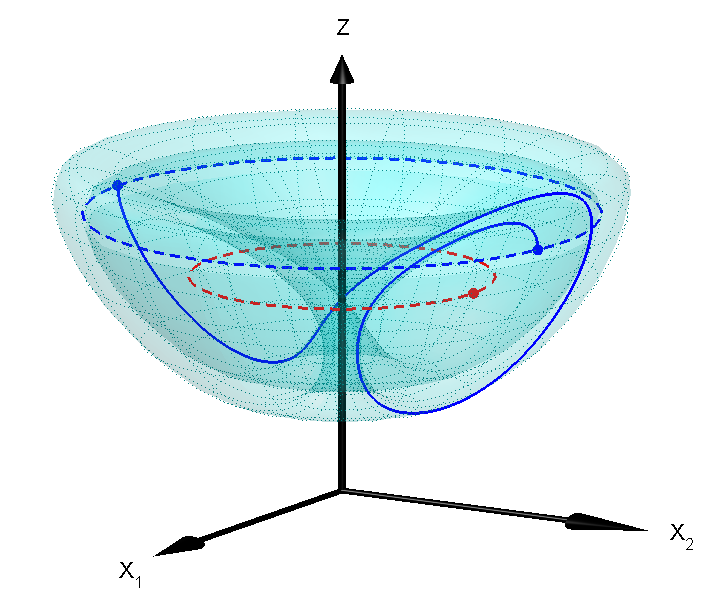
\includegraphics[width=0.35\textwidth,clip=true]{01grouporbit}
\end{center}
  \caption
  [\CLf: $\cycle{01}$ {\rpo} group orbit]{
  \CLf: The relative equilibrium $TW_1$ is shown by the red dot. The dashed red
  line shows its group orbit, which as a relative equilibrium is also its
  temporal evolution. One period of the $\cycle{01}$ {\rpo} is
  shown by the solid blue line. The group orbit of its starting point
  is shown by the dashed blue line and it can be seen that after one
  period it has returned to the same group orbit but with a different phase. The
  group orbit of the temporal orbit of the dark blue trajectory is shown by the
  cyan surface. Also (barely) visible are 15 more periods of $\cycle{01}$, which
  are shown by the faint dotted lines. It can be seen that these orbits lie on
  the torus generated by the group orbit of the first period.}
\label{fig:CLf01group}
\end{figure}


\subsection{Pipes and planes}

 %% A27*-pipeSymms.* - read dasbuch/book/FigSrc/inkscape/00ReadMe.txt
 \begin{figure}
 \begin{center}
  \setlength{\unitlength}{0.20\textwidth}
  %% \unitlength = units used in the Picture Environment
(a)
  \begin{picture}(1,0.52454249)%
    \put(0,0){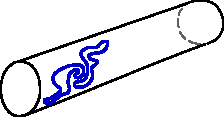
\includegraphics[width=\unitlength]{A27a-pipeSymms}}%
    \put(0.61583231,0.13683004){\color[rgb]{0,0,0}\makebox(0,0)[lb]{\smash{$z$}}}%
    \put(0.00611823,0.27217453){\color[rgb]{0,0,0}\makebox(0,0)[lb]{\smash{$\theta$}}}%
  \end{picture}%
(b)
  \begin{picture}(1,0.52454249)%
    \put(0,0){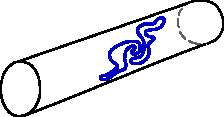
\includegraphics[width=\unitlength]{A27b-pipeSymms}}%
    \put(0.61583231,0.13683004){\color[rgb]{0,0,0}\makebox(0,0)[lb]{\smash{$z$}}}%
    \put(0.00611823,0.27217453){\color[rgb]{0,0,0}\makebox(0,0)[lb]{\smash{$\theta$}}}%
  \end{picture}%
\\
(c)
  \begin{picture}(1,0.52454249)%
    \put(0,0){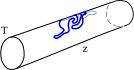
\includegraphics[width=\unitlength]{A27c-pipeSymms}}%
    \put(0.61583231,0.13683004){\color[rgb]{0,0,0}\makebox(0,0)[lb]{\smash{$z$}}}%
    \put(0.00611823,0.27217453){\color[rgb]{0,0,0}\makebox(0,0)[lb]{\smash{$\theta$}}}%
  \end{picture}%
(d)
  \begin{picture}(1,0.52454249)%
    \put(0,0){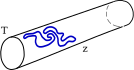
\includegraphics[width=\unitlength]{A27d-pipeSymms}}%
    \put(0.61583231,0.13683004){\color[rgb]{0,0,0}\makebox(0,0)[lb]{\smash{$z$}}}%
    \put(0.00611823,0.27217453){\color[rgb]{0,0,0}\makebox(0,0)[lb]{\smash{$\theta$}}}%
  \end{picture}%
 \end{center}
 \caption{\label{fig:A27-pipeSymms}
$\On{2}_\theta \times \SOn{2}_z$ symmetry of flow in a stream-wise
periodic pipe: A \rpo\ $p$ is a state of the fluid
 (a)
that reappears
 (b)
period $\period{}$ later, translated by downstream shift $\shift$
(in contrast to a \reqv, a constant shape that travels
downstream with constant {\phaseVel} $\velRel$); such solutions are
stream-wise $\SOn{2}_z$ equivariant; or
 (c)
period $\period{}$ later, translated by downstream shift $\shift$ and
rotated azimuthaly by $\gSpace_p$; $\SOn{2}_{\theta} \times \SOn{2}_z$
equivariant; or
 (d)
period $\period{}$ later, reflected and rotated azimuthaly by
$\gSpace$; $\On{2}_{\theta}$ equivariant
(from \wwwcb{}).
 }%
 \end{figure}
													\toCB
    \PC{emphasize that our turbulent states are \emph{not} localized
    three-dimensional solitary waves as quasi-particles -
    \reffig{fig:A27-pipeSymms} might be misleading. Our solutions are
    global, distributed over the whole volume.}
The symmetry group $\Gpipe$ of stream-wise periodic pipe flow contains
two commuting \SOn{2} rotations (\reffig{fig:A27-pipeSymms}). Each
\SOn{2} group orbit is topologically a circle
(\reffig{fig:2840GOt135th0}), and together they sweep out a contorted
$T^2$ torus (\reffig{fig:2830GO6}).

\subsection{\CLe}


\section{Group action}

\subsection{Group orbit}

\subsection{Finite shifts}

\subsection{Eqs of motion}
\subsection{Infinitesimal, Jacobian derivative}
\subsection{Moving frame}

%%%%%%%%%%%%%%%%%%%%%%%%%%%%%%%%%%%%%%%%%%%%%%%%%
% 2011-09-09, 2012-03-30 Predrag: add BeThMovFr to
%            continuous.tex overheads, and ChaosBook
% replace A27movFrame*.* everywhere
\begin{figure}
 \begin{center}
  \setlength{\unitlength}{0.20\textwidth}
  %% \unitlength = units used in the Picture Environment
(a)~~
  \begin{picture}(1,0.98655417)%
    \put(0,0){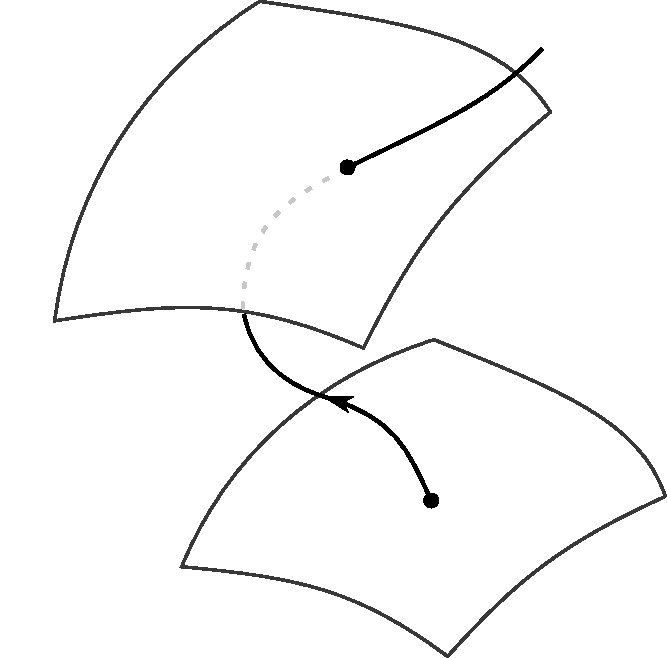
\includegraphics[width=\unitlength]{BeThTrajTeX}}%
    \put(0.35976094,0.91875614){\color[rgb]{0,0,0}\rotatebox{-31.32889204}{\makebox(0,0)[lb]{\smash{$\pS_{\ssp(\zeit)}$}}}}%
        \put(0.60333631,0.42274457){\color[rgb]{0,0,0}\rotatebox{-40.8073288}{\makebox(0,0)[lb]{\smash{$\pS_{\ssp(0)}$}}}}%
    \put(0.66001383,0.16959019){\color[rgb]{0,0,0}\rotatebox{0.0313674}{\makebox(0,0)[lb]{\smash{$\ssp(0)$}}}}%
    \put(0.5058276,0.64524238){\color[rgb]{0,0,0}\rotatebox{0.0313674}{\makebox(0,0)[lb]{\smash{$\ssp(\zeit)$}}}}%
    \put(0.13110825,0.05766516){\color[rgb]{0,0,0}\rotatebox{0.11031334}{\makebox(0,0)[lb]{\smash{$\pS$}}}}%
  \end{picture}%
~~(b)
  \begin{picture}(1,0.98655417)%
    \put(0,0){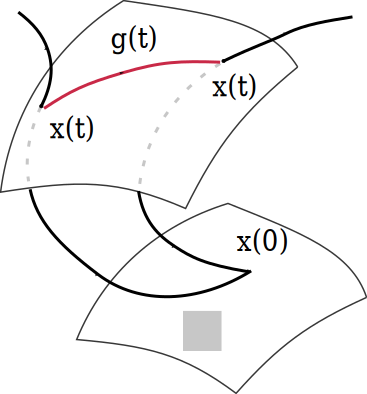
\includegraphics[width=\unitlength]{BeThMovFr}}%
    \put(0.20559239,0.64023845){\color[rgb]{0,0,0}\rotatebox{0.0313674}{\makebox(0,0)[lb]{\smash{$\ssp(\zeit)$}}}}%
    \put(0.67382401,0.35781161){\color[rgb]{0,0,0}\rotatebox{0.0313674}{\makebox(0,0)[lb]{\smash{$\ssp(0)$}}}}%
    \put(0.61221026,0.74589514){\color[rgb]{0,0,0}\rotatebox{0.0313674}{\makebox(0,0)[lb]{\smash{$\sspRed(\zeit)$}}}}%
    \put(0.35760559,0.8662057){\color[rgb]{0,0,0}\rotatebox{0.0313674}{\makebox(0,0)[lb]{\smash{$\LieEl(\zeit)$}}}}%
  \end{picture}%
 \end{center}
  \caption{\label{fig:BeThMovFr}
(a)
The group orbit $\pS_{\ssp(0)}$ of \statesp\ point $\ssp(0)$, and the
group orbit $\pS_{\ssp(\zeit)}$ reached by the trajectory $\ssp(\zeit)$ time $t$
later.
(b)
The two physically equivalent flows $\ssp(\zeit)=\LieEl(\zeit)\,\sspRed(\zeit)$ are related
by, in general, an arbitrary, time dependent {\em moving frame} transformation $\LieEl(\zeit)$.
(from \wwwcb{}).
  }
\end{figure}
%%%%%%%%%%%%%%%%%%%%%%%%%%%%%%%%%%%%%%%%%%%%%%%%%%

													\toCB
    \PC{
Use \reffig{fig:A27movFrame} in ChaosBook.org and siminos/atlas/atlas.tex.
(to Predrag: remember to copy them to dabook/book/Fig and FigSrc/).
How it was drawn is described in
dasbuch/book/FigSrc/inkscape/00ReadMe.txt
    }

\subsection{Relative invariant solutions}
\label{s:RelInvSol}

Along with continuous symmetries come important classes of invariant
solutions referred to as `relative' or `equivariant'
\rf{Huyg1673,Poinc1896}. One expects to find relative
equilibria and \rpo s\rf{Rand82}, associated with the translational
and rotational symmetries of the flow.

A {\em \reqv} is a dynamical
orbit whose velocity field %DB:4/9 this equation \refeq{symbolicNS} doesn't exist in the paper anymore
lies within the group tangent space, with a constant phase speed $c$,
% $c=(c_1,\cdots,c_N)$,
and whose time evolution is thus confined to the group orbit, i.e.,
\bea
\vel(\ssp) &=& c \, \groupTan(\ssp) % c \cdot \groupTan(\ssp)
\label{phaseVel}\\
\ssp(\zeit) &=& \LieEl(\gSpace(\zeit)) \, \ssp(0)
%          = \mathrm{e}^{ \zeit  c \Lg} \,  \ssp(0)
%           = \mathrm{e}^{ \zeit\,  c \cdot \Lg} \,  \ssp(0)
\,,\qquad
\ssp(\zeit) \in \pS_{\REQV{}{}}
\nnu
\,.
\eea
While in the case of \SOn{2} symmetry a \reqv\ traces out a loop in the
full \statesp (see Fig. \ref{fig:CLf01group}, e.g.), for a higher-dimensional continuous symmetry it explores
the group orbit $\pS_{\REQV{}{}}$ quasi-periodically, so a \reqv\ is
\emph{not} a \po. Rather, as all states in this group orbit are
physically the same state for all time, this is a generalized \eqv\ state. Depending on the context, \reqva\ can also be called travelling waves and
rotational waves.

A {\rpo} $p$ is an orbit in {\statesp} $\pS$ which exactly recurs
\[ %beq
\ssp(\zeit) = \LieEl_p \, \ssp(\zeit + \period{p} )
    \,,\qquad
\ssp(\zeit) \in \pS_p
\] %ee{RPOrelper1}
after a fixed {relative period} $\period{p}$, but shifted by a fixed group
action ${\LieEl}$ that maps the endpoint $\ssp (\period{} ) $ back
into the initial point cycle point $\ssp (0) $ (see Fig. \ref{fig:CLf01group} for an example in \CLf).

Continuous symmetry parameters (`phases' or `shifts')
$\{\gSpace_j\}=\{\phi_p,\shift_p\}$
% $\{\gSpace_1,\cdots,\gSpace_N\}$
are real numbers, ratios $\pi/\gSpace_j$ are almost never rational, and
\rpo s are almost never eventually periodic; the time evolution
of a relative periodic point thus sweeps out quasi-periodically the
$3$\dmn\ group orbit $\pS_p$ without ever closing into a \po, unless the
dynamics is restricted to a discrete-symmetry invariant subspace.

Visualizing a single `relative' orbit in its co-moving frame is useful if
we are concerned with that individual solution. Unfortunately, it is
useless if we are concerned with studying collections of these orbits
since different orbits do not share the same co-moving frame.

In a co-moving frame, moving with the mean phase velocity of a given
solution, a \rpo\ reduces to a \po.
However, as each solution travels with its own mean phase velocity,
there is no single co-moving frame that can simultaneously reduce
\emph{all} traveling solutions. % DB: Removed "downstream" to take focus away from fluid dynamics.
